\chapter{Background and related work}

\section{Language, social Identity and stereotyping}

\textbf{Background}
\begin{itemize}
    \item Origin of bias (System -1 and system -2) ; TWO FAMILIES OF COGNITIVE OPERATIONS \cite{kahneman2002representativeness}
    \item  How stereotypes are inevitably formed (implicit bias) ??
    Impressions + labels ...
    \cite{fiske1998stereotyping}
    \item Difference between stereotype and prejudice \cite{fiske1998stereotyping}
    \begin{itemize}
        \item Stereotype (Cognitive) : An overgeneralized belief about a particualr group of people.This need not be negative but sometimes be accurate, like Lions have four legs. But the problem arises if the stereotype is rooted with inaccurate association formed between target from social groups (gender, ethnicity ..) and its attribute. 
        \item Prejudice (Attitude) : "pre-judgement", typically negative attitude towards an individual or group.
        \item Discrimination (Behaviour) : Stereotypical beliefs combined with prejudicial attitude towards social groups can drive the behavior to change which results in discrimination.\label{crashcrouse}\footnote {\url{https://www.youtube.com/watch?v=7P0iP2Zm6a4&ab_channel=CrashCourse}}
    \end{itemize}
\end{itemize}
\textbf{Perspectives of stereotypes}
\begin{itemize}
        \item Stereotypes cannot be avoided, as they are implicitly formed as a part of the cognitive process. When these associations/ implicit bias (deviation from rationality) are overgeneralized followed by, this leads to stereotyping. Hence arises two perspectives or dimensions of stereotypes 
            \begin{itemize}
                \item Stereotypes (as pictures in head / Implicit associations)
                \item Stereotyping (Socially shared Stereotypical associations / Overgeneralized beliefs and expectancies) 
            \end{itemize}
            \item Coming to this thesis, social stereotypes are being studied where the focus is mainly on examining 
            \begin{itemize}
                \item Biased stereotypical associations
                \item Socially shared Stereotypes
            \end{itemize}
\end{itemize}
\begin{itemize}
    \item Describe two perspective, Stereotypes as pictures in head and stereotyping (shared social beliefs and expectancies)
    \item Definitions of stereotype from other papers
        \begin{itemize}
            \item Stereotypes definition taxonomy \cite{ashmore1981conceptual}
        \end{itemize}
    \item Cognitive processes in stereotyping and intergroup behavior \cite{hamilton2015cognitive}
    \item Stereotypes and stereotyping \cite{macrae1996stereotypes}
    \item Prescriptive and descriptive stereotyping
    \item Types of harms caused by bias [Kate Crawford. 2017. The Trouble with Bias. Keynote
at NeurIPS]
\end{itemize}
\textbf{How language contributes to stereotype formation}
    \begin{itemize}
        \item Stereotypes as collective belief systems \cite{macrae1996stereotypes}
        \item How language contributes to stereotype formation \cite{burgers2020language}
        \item How stereotypes are shared through language: a
    review and introduction of the social categories
    and stereotypes communication (SCSC) framework \cite{beukeboom2019stereotypes}
    \end{itemize}
\section{Machine learning and deep learning}
\subsection{Machine learning pipeline}
    \begin{itemize}
        \item Machine learning setup by abu mustafa 
        \begin{figure}[t]
            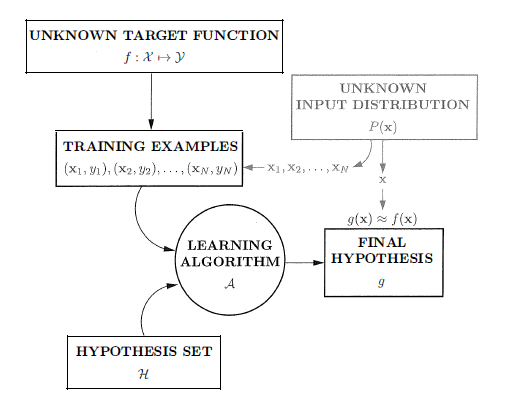
\includegraphics[width=8cm]{thesis/figures/Learning problem.PNG}
            \centering
            \caption{The learning problem setup}
            \label{fig:The learning problem setup}
        \end{figure}
        \begin{enumerate}
            \item Explain different components of learning problem  learning problem 
            
        \end{enumerate}
        \item Types of training (supervised, unsupervised, reinforcement learning and focus on supervised)
        \item Learning models (Classification, regression)
        \item Linear and logistic Regression and gradient descent 
        \textbf{Refer to udemy machine learning course notes}
        % \item SVM and selected classifiers \textbf{TBD ??}
    \end{itemize}
\subsection{Neural Networks architecture}
    \begin{itemize}
        \item Deep learning vs Machine learning 
        \item Neural network basic setup (perceptron learning algorithm)
        \item Basic neural network forward pass and backward pass
        \item  Deep neural network and its variants
        \item Refer \url{https://github.com/mvdheram/DeepLearning-Notebooks/blob/main/Introduction_to_PyTorch.ipynb}
        \item \textbf{IMP : Classification using neural networks} 
    % \end{itemize}
    % \begin{itemize}
        \item Dropout for regularization 
    \end{itemize}
\subsection { Recurrent Neural Networks }
            \begin{itemize}
                \item Limitations of NN 
                \item Why RNN when dealing with text ?
                \item Contextual word embedding
            \end{itemize}

\subsection{Transformer architecture}
    
\section{Natural language processing and language modeling}
    \subsection{Vector representation of text}
    \begin{itemize}
        \item What is NLP?
        \item Feature vectors for text 
            \begin{itemize}
                \item Bag of words
                \item TF-IDF
            \end{itemize}
        \item Word embeddings
        \item Static word embedding
        \item Word2vec, glove basic architecture
        \item Text classification 
        \begin{itemize}
            \item classification types (Binary, multi class, multi label)
            \item LPP
            \item Sigmoid activation function and binary cross entropy loss function
        \end{itemize}
    \end{itemize}
    \subsection{Language modeling}
    \subsection{Transfer learning}
    \subsection{BERT architecture}
% \section {Evaluation metrics}    
\section{Bias and social bias in Natural language processing}
\begin{itemize}
    \item A critical survey of bias in NLP \cite{blodgett2020language}
    \item A survey on Bias in Deep NLP \cite{garrido2021survey}
\end{itemize}